% Asset ID: A22FurtherKinematicsTikZ-003
% Unit: A22
% Topic: Further Kinematics
% Related section: Speed and bearing
\documentclass[tikz,border=8pt]{standalone}
\usepackage{amsmath}
\usetikzlibrary{arrows.meta,positioning,angles,quotes}
\begin{document}

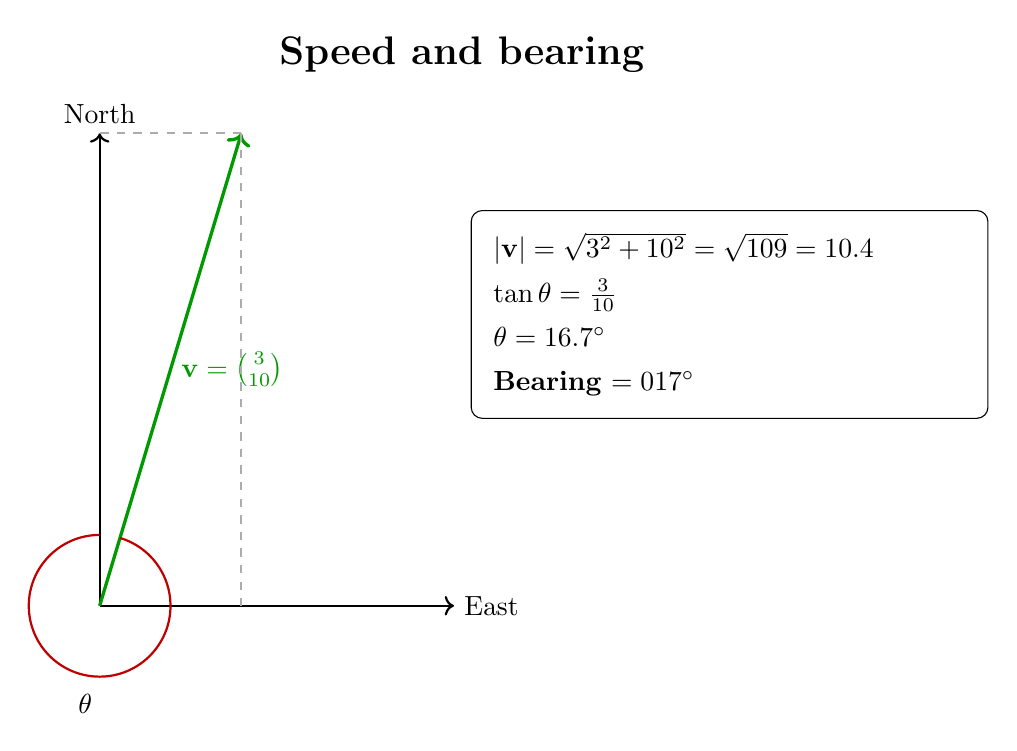
\begin{tikzpicture}[axis/.style={->, thick}, velocity/.style={->, very thick, green!60!black}, helper/.style={gray!65, thick, dashed}, box/.style={draw,rounded corners,fill=white,align=left,inner sep=8pt}]
\node[font=\bfseries\Large] at (4.6,7) {Speed and bearing};
\coordinate (O) at (0,0); \coordinate (N) at (0,6); \coordinate (E) at (4.5,0); \coordinate (V) at (1.8,6);
\draw[axis] (O)--(N) node[above]{North}; \draw[axis] (O)--(E) node[right]{East};
\draw[velocity] (O)--(V) node[midway,right] {$\mathbf v=\binom{3}{10}$};
\draw[helper] (V)--(1.8,0); \draw[helper] (V)--(0,6);
\pic [draw=red!75!black, thick, "$\theta$", angle eccentricity=1.4, angle radius=0.9cm] {angle = N--O--V};
\node[box, text width=6cm] at (8,3.7) {$|\mathbf v|=\sqrt{3^2+10^2}=\sqrt{109}=10.4$\\[4pt]$\tan\theta=\frac{3}{10}$\\[4pt]$\theta=16.7^\circ$\\[4pt]\textbf{Bearing }$=017^\circ$};
\end{tikzpicture}
\end{document}
